\documentclass[utf8]{beamer}

\usepackage{pgfpages}
\usepackage{beamerthemesplit}
\usepackage{latexsym}
\usepackage{eurosym}
\usepackage[english]{babel}
\usepackage{ae,aecompl}
\usepackage{graphicx}
\usepackage{amsfonts}
\usepackage{verbatim}
\usepackage{times}
\usepackage[T1]{fontenc}
\usepackage{listings}
\usepackage{multirow}
\usepackage{amsmath}

%\setbeameroption{show notes on second screen}
%\setbeameroption{show only notes}

%Configuracion paquete listings
\definecolor{gris}{rgb}{0.9,1.0,1.0}
\definecolor{gris2}{rgb}{0.9,0.9,0.9}
\definecolor{gray90}{gray}{.90}
\definecolor{gray97}{gray}{.97}
\definecolor{gray75}{gray}{.75}
\definecolor{gray45}{gray}{.45}
\lstset{ %
    %frame=Lpb,                        % adds a frame around the code
    framerule=0pt,
    aboveskip=0.5cm,
    framextopmargin=3pt,
    framexbottommargin=3pt,
    framexleftmargin=0.4cm,
    framesep=0pt,
    rulesep=.4pt,
    % backgroundcolor=\color{gray97},
    rulesepcolor=\color{black},
    texcl=true,
    %
    stringstyle=\ttfamily,
    showspaces=false,               % show spaces adding particular underscores
    showstringspaces=false,         % underline spaces within strings
    showtabs=false,                 % show tabs within strings adding particular underscores
    tabsize=2,                      % sets default tabsize to 2 spaces
    captionpos=b,                   % sets the caption-position to bottom
    basicstyle=\footnotesize,       % the size of the fonts that are used for the code
    commentstyle=\color{gray45},
    keywordstyle=\bfseries,
    breakatwhitespace=false,        % sets if automatic breaks should only happen at whitespace
    %
    %numbers=left,
    %numbersep=5pt,                  % how far the line-numbers are from the code
    %numberstyle=\tiny,              % the size of the fonts that are used for the line-numbers
    %numberfirstline = false,
    breaklines=true,
}

%% Define a new 'leo' style for the package that will use a smaller font.
\makeatletter
\def\url@leostyle{%
  \@ifundefined{selectfont}{\def\UrlFont{\sf}}{\def\UrlFont{\sf}}}
\makeatother
%% Now actually use the newly defined style.
\urlstyle{leo}


\usetheme{CambridgeUS}
\usecolortheme{dolphin}
\setbeamertemplate{navigation symbols}{}
\setbeamertemplate{footline}
{
  \leavevmode%
  \hbox{%
  \begin{beamercolorbox}[wd=.333333\paperwidth,ht=2.25ex,dp=1ex,center]{author in head/foot}%
    \usebeamerfont{author in head/foot}\insertshortauthor
  \end{beamercolorbox}%
  \begin{beamercolorbox}[wd=.666666\paperwidth,ht=2.25ex,dp=1ex,center]{title in head/foot}%
    \usebeamerfont{title in head/foot}\insertshorttitle
  \end{beamercolorbox}
  }
  \vskip0pt%
}
\setbeamercolor{titlelike}{parent=structure,bg=gray90}
\setbeamercolor{block body}{bg=gray90}
\setbeamercolor{block title}{bg=gray75}

\title{Ley de Amdahl para multicore}
\subtitle{MICAP ATC 2012-2013}
\author[]{Daniel Ampuero Anca \\ Daniel Fernández Nuñez \\ Isaac Fernández Varela \\ Juan Font Alonso}

\date[7 de enero de 2012] % (optional, should be abbreviation of conference name)


%%%%%%%%%%%%%%%%%%%%%%%%%%%%%%%%%%%%%%%%%%%%%%%%%%%%%%%%%%%%%%%%%%%%%%%%%%%%%%%%

\begin{document}

\renewcommand{\figurename}{Figura} 


\begin{frame}
    \maketitle
\end{frame}

\section*{Indice}
\subsection*{Indice}
\begin{frame}
    \tableofcontents
\end{frame}

%%%%%%%%%%%%%%%%%%%%%%
\section{Ley de Amdahl}
%%%%%%%%%%%%%%%%%%%%%%

\subsection*{Ley de Amdahl}
%%%%%%%%%%%%%%%%%%%%%%%%%%%%%%%%%%%

\begin{frame}[allowframebreaks]{Ley de Amdahl}
    \begin{block}{Gene Amdahl, 1967}
        La mejora obtenida en el rendimiento de un sistema debido a la alteración de uno de sus componentes está limitada por la fracción de tiempo que se utiliza dicho componente
    \end{block}
    \begin{block}{Ecuación}
        $$ T_{mejora} = T_{orginal} * (1 - F_{mejora} + \frac{F_{mejora}}{A_{mejora}}) $$
        \begin{itemize}
            \item $T_{mejora}$: tiempo total tras mejorar una parte del programa.
            \item $T_{original}$: tiempo antes de la mejora.
            \item $F_{mejora}$: fracción del total de la parte que se mejora.
            \item $A_{mejora}$: aceleración que se consigue en la parte mejorada.
        \end{itemize}
    \end{block}
    \begin{block}{Cálculo de la aceleración}
        $$ A = \frac{T_{original}}{T_{mejora}} = \frac{1}{1-F{mejora}+\frac{F_{mejora}}{A_{mejora}}} $$
        \begin{itemize}
        \item Si $A_{mejora} \rightarrow \infty$ entonces $A = \frac{1}{1 - F_{mejora}}$ \\
        \item La aceleración siempre está limitada por la fracción de programa que se puede mejorar.
        \end{itemize}
    \end{block}
    \begin{block}{Ejemplos}
        \begin{itemize}
        \item ¿Cuál es la aceleración total de un programa si una porción de código del 75 \% va 2 veces más rápido?
        $$ A = \frac{1}{1-F{mejora}+\frac{F_{mejora}}{A_{mejora}}} = \frac{1}{1 - 0.75 + \frac{0.75}{2}} = \frac{1}{0.625} = 1.6 $$
        \item ¿Cuál es la máxima aceleración posible si se puede mejorar el 90 \% del código?
        $$ A = \frac{1}{1 - F_{mejora}} = \frac{1}{1 - 0.9} = 10 $$
        \end{itemize}
    \end{block}
    \begin{block}{Representación gráfica}
        \begin{figure}[htp]
            \begin{center}
            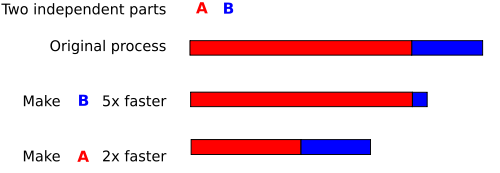
\includegraphics[width=.7\linewidth]{amdahl}
            \caption{Explicación gŕafica de la Ley de Amdahl}
            \label{fig:amdahl}
            \end{center}
        \end{figure}
    \end{block}
    \begin{block}{Extensión de Amdahl para multicore}
        \begin{itemize}
            \item Suponiendo $n$ cores
            \item Suponiendo una fracción de código paralelizable $F_{paralelizable}$
            \item Descartando penalizaciones de la paralelización
            $$ A = \frac{1}{1 - F_{mejora} + \frac{F_{mejora}}{n}} $$
        \end{itemize}
    \end{block}
    \begin{block}{Problemas de la extensión de Amdahl}
        \begin{itemize}
            \item Demasiado simplificada.
            \item ¿Todos los multicores son iguales?
        \end{itemize}
    \end{block}
\end{frame}

%%%%%%%%%%%%%%%%%%%%%%%%%%%%%%%%%%%%%%%%%%%%%%%%%%%%%%%%%%%%%%
\section{Ley de Amdahl en multicore}
%%%%%%%%%%%%%%%%%%%%%%%%%%%%%%%%%%%%%%%%%%%%%%%%%%%%%%%%%%%%%%

\subsection*{Estructura de los multicore}
%%%%%%%%%%%%%%%%%%%%%%%%%%%%%%%%%%%%%%%%%%%%%%%%%%

\begin{frame}[allowframebreaks]{Definición de un chip multicore}
    \begin{block}{\emph{Baseline Core Equivalent}}
        \begin{itemize}
        \item Podemos suponer una unidad lógica teórica para definir los cores.
        \item Unídad mínima funcional con rendimiento $perf(BCE) = 1$
        \item Los cores de un chip se forman agrupando $r$ BCE con rendimiento $perf(r)$
        \item Un chip está formado por $n$ BCE agrupados en cores.
        \end{itemize}
    \end{block}
    \begin{block}{Rendimiento de un core}
        \begin{itemize}
            \item Se define la función $perf(r)$ para el rendimiento de un core de $r$ BCE.
            \item $perf(r) = r^y, 0 < y < 1$
            \item Normalmente se utiliza $y = \frac{1}{2}, perf(r) = \sqrt{r}$
        \end{itemize}
    \end{block}
    \begin{block}{Configuración de un multicore}
        \begin{itemize}
        \item Según como se agrupen los $n$ BCE de un chip podemos definir los tipos de multicore:
            \begin{itemize}
                \item \textbf{Simétrico:} $n$ BCE en grupos de $r$ para formar $\frac{n}{r}$ cores.
                \item \textbf{Asimétrico:} un core de $r$ BCE y $n - r$ cores con un único BCE.
                \item \textbf{Dinámico:} un core con varios BCE, pudiendo cambiar el número de BCE dinámicamente. El resto de BCE no se agrupan formando cada uno un core.
            \end{itemize}
        \end{itemize}
    \end{block}
\end{frame}

\subsection*{Ley de Amdahl en multicores}

\begin{frame}{Amdahl en multicores simétricos}
    \begin{block}{Ley de Amdahl}
        \begin{itemize}
        \item Teniendo un procesador con $n$ cores con $r$ BCE por core.
        $$ Speedup_{symmetric} = \frac{1}{\frac{1 - f}{perf(r)} + \frac{f  r}{perf(r)  n}} $$
        \item La parte secuencial $(1 - f)$ se ve influenciada por el rendimiento de un core $perf(r)$
        \item La parte paralela $(f)$ varía con el rendimiento de todos los cores, $\frac{n}{r}perf(r)$
        \end{itemize}
    \end{block}
\end{frame}

\begin{frame}[allowframebreaks]{Amdahl en multicores asimétricos}
    \begin{block}{Ley de Amdahl}
        \begin{itemize} 
            \item Un core con rendimiento $perf(r)$ y $n - r$ cores con rendimiento 1.
            $$ Speedup_{assymetric} = \frac{1}{\frac{1 - f}{perf(r)} + \frac{f}{perf(r) + n - r}} $$
            \item La parte secuencial de nuevo viene marcada por un único core con rendmiento $perf(r)$
            \item La parte paralela mejorará con la suma de rendimiento de todos los cores, $perf(r) + perf(BCE) (n - r) = perf(r) + n - r$
        \end{itemize}
    \end{block}
    \begin{block}{Ventajas}
        \begin{itemize}
            \item El rendimiento puede ser mayor que el de las configuraciones simétricas, nunca inferior.
            \item Se beneficia de acelerar la parte secuencial al mismo tiempo que la paralela.
        \end{itemize}
    \end{block}
\end{frame}

\begin{frame}[allowframebreaks]{Amdahl en multicores dinámicos}
    \begin{block}{Ley de Amdahl}
        \begin{itemize}
            \item $n$ cores con la posibilidad de que uno reclame $r$ BCE en algún momento.
            $$ Speedup_{dynamic} = \frac{1}{\frac{1 - f}{perf(r)} + \frac{f}{n}} $$
            \item En la parte secuencial se reclamarán $r$ BCE ejecutándose con un rendimiento $perf(r)$
            \item En la parte paralela se utilzárán los $n$ cores de un BCE con un rendimiento $n\,perf(BCE) = n$
        \end{itemize}
    \end{block}
    \begin{block}{Ventajas e inconvenientes}
        \begin{itemize}
            \item El rendimiento puede ser mayor que el de las configuraciones asimétricas, nunca inferior.
            \item Cambiar dinámicamente el número de cores le permite optimizar la aceleración tanto en secuencial como en paralelo. 
            \item No es fácil implementarlos a nivel hardware.
        \end{itemize}
    \end{block}
\end{frame}

%%%%%%%%%%%%%%%%%%%%%%%%%%%%%%%%%%%%%%%%%%%%%%%%%%%%%%%%%%%%%%
\section{Extensiones a la ley de Amdahl}
%%%%%%%%%%%%%%%%%%%%%%%%%%%%%%%%%%%%%%%%%%%%%%%%%%%%%%%%%%%%%%


\begin{frame}{Ley de Amdahl}
    \begin{block}{}
    \begin{itemize}
        \item Según la ley de Amdahl multicore, el procesamiento en paralelo no es escalable debido a la fracción secuencial.
        \item Si una aplicación es paralelizable al 90\%, con 8-16 procesaodres, el 10\% secuencial contribuirá al 50-80\% del tiempo.
        \item Por ello, la ley de Amdahl se considera un modelo de speedup a tamaño fijo (\emph{fixed-size})
        \item Otro concepto: modelo de speedup a tiempo fijo (\emph{fixed time}): \textbf{Ley de Gustafson}.
    \end{itemize}
    \end{block}
\end{frame}

\subsection*{Ley de Gustafson}

\begin{frame}[allowframebreaks]{Ley de Gustafson}
    \begin{block}{Argumentación}
        \begin{itemize}
            \item Máquinas más potentes están diseñadas para problemas grandes.
            \item El problema también debe escalar en proporción.
        \end{itemize}
    \end{block}
    \begin{block}{Ley de Gustafson}
        \begin{itemize}
            \item \emph{Fixed-Time Speedup}
            $$ Speedup_{FT} = (1 - f) + mf $$
            \item Siendo $f$ la fracción paralela y $m$ el número de cores.
            \item No contradice la ley de Amdahl: es una observación de que los supuestos de Amdahl no coinciden con la forma en la que se usan los multicore
        \end{itemize}
    \end{block}
    \begin{block}{Escalabilidad del speedup}
        Speedup con ley de Amdahl vs Speedup con ley de Gustafson
    \end{block}
    \begin{center}
        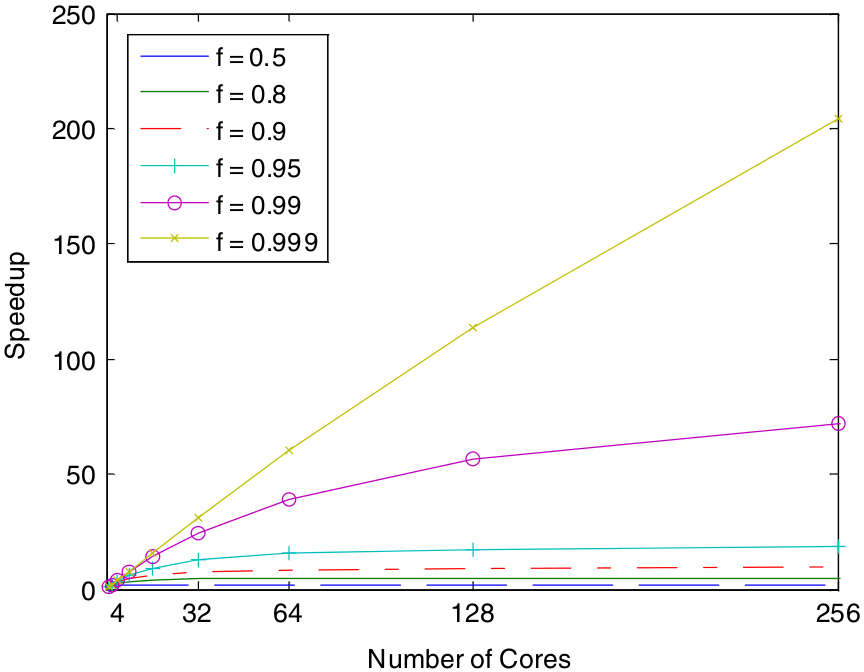
\includegraphics[width=.5\linewidth]{figures/fixedsize_speedup}
        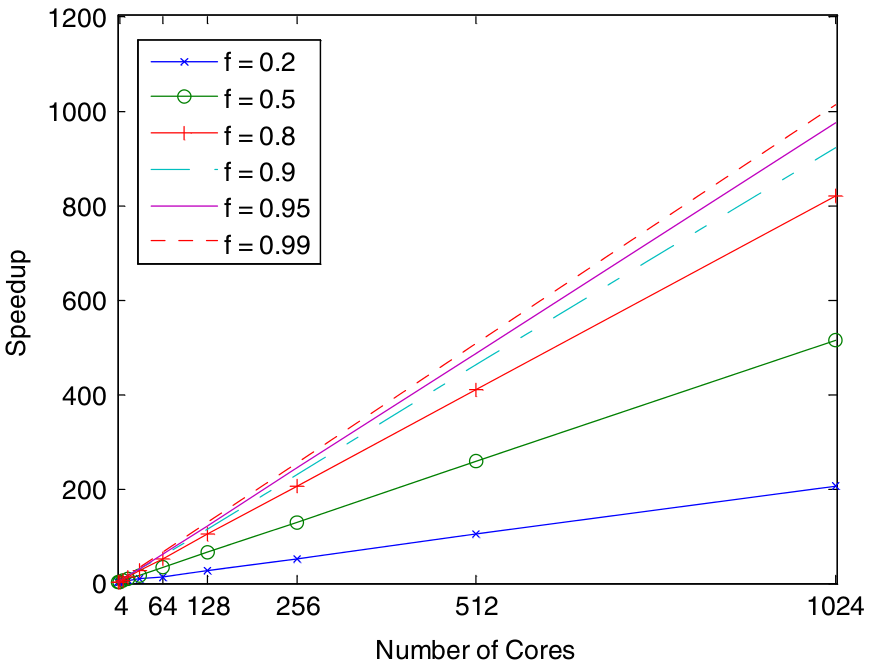
\includegraphics[width=.5\linewidth]{figures/fixedtime_speedup}
    \end{center}
\end{frame}

\subsection*{Speedup ligado a memoria}

\begin{frame}[allowframebreaks]{Speedup ligado a memoria}
    \begin{block}{Limitación por memoria}
        \begin{itemize}
        \item Las leyes de Amdahl y Gustafson son simplistas: no tienen en cuenta limitaciones físicas.
        \item En la práctica, el componente físico que más afecta la computación es la memoria.
        $$ Speedup_{MemoryBounded} = \frac{(1-f) + f \bar{g}(m)}{(1-f) + \frac{f\bar{g}(m)}{m}} $$
        \end{itemize}
    \end{block}
    \begin{block}{$\bar{g}(m)$}
        \begin{itemize}
	    \item $m$ = número de cores
            \item $\bar{g}(m)$ es una función específica para cada algoritmo que depende de la relación entre el número de operaciones de computación y de las operacioens en memoria.
            \item Generalización de las leyes anteriores:
            \begin{itemize}
                \item Ley de Amdahl: $\bar{g}(m) = 1$
                \item Ley de Gustafson: $\bar{g}(m) = m$
            \end{itemize}
        \end{itemize}
    \end{block}
    \begin{block}{Algoritmo ejemplo: multiplicación de matrices}
        \begin{itemize}
            \item Operaciones de cómputo: $2N^3$
            \item Operaciones en memoria: $3N^2$
            \item Se obtiene una $\bar{g}(x) = x^\frac{3}{2}$
            $$ Speedup_{MB} = \frac{(1-f) + f \bar{g}(m)}{(1-f) + \frac{f\bar{g}(m)}{m}} = \frac{(1-f) + f m^\frac{3}{2}}{(1-f) + fm^\frac{1}{2}} $$
        \end{itemize}
    \end{block}
    \begin{block}{Speedup alcanzado}
        \begin{itemize}
            \item Como en el ejemplo, si $\bar{g}(m) > m$ el speedup ligado a memoria es mayor que el correspondiente al de la ley de Gustafson.
                \begin{itemize}
                    \item Algoritmos con accesos a memoria optimizados y buen aprovechamiento de las cachés.
                \end{itemize}
        \end{itemize}
    \end{block}
    \begin{block}{Resultados}
        Speedup ligado a memoria y comparativa con el resto de leyes
    \end{block}
    \begin{center}
        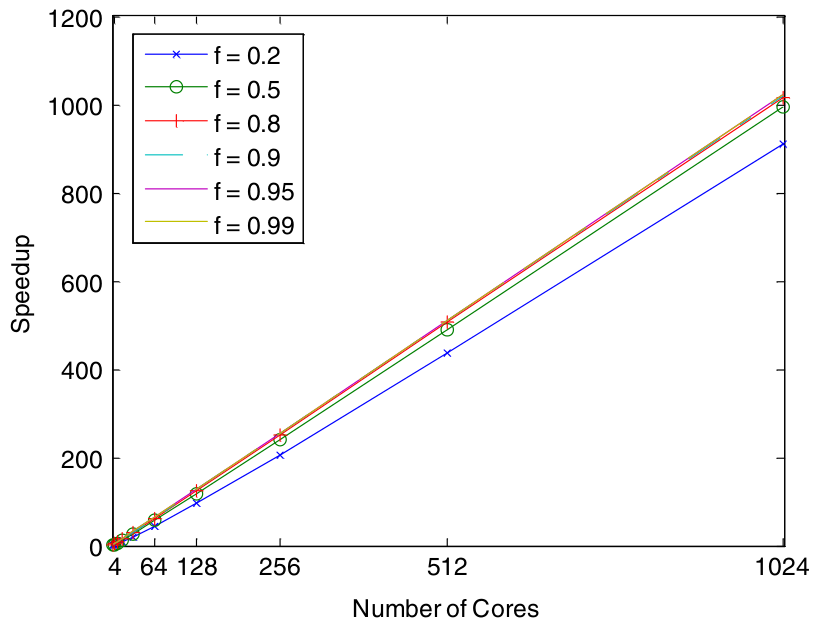
\includegraphics[width=.5\linewidth]{figures/mb_speedup}
        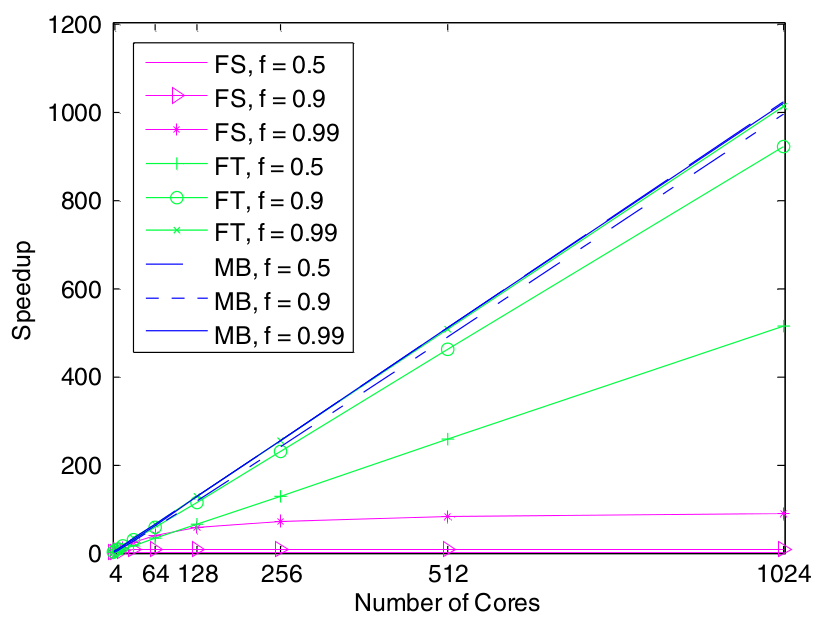
\includegraphics[width=.5\linewidth]{figures/all_speedups}
    \end{center}
\end{frame}

\begin{frame}{Limitaciones de la memoria}
    \begin{block}{Conclusión}
        En el área de la computación escalable, el procesamiento secuencial no es el factor limitante.
        \begin{itemize}
        \item Sin embargo, existen problemas para alcanzar los speedups teóricos en los multicore
        \end{itemize}
    \end{block}
    \begin{columns}
        \begin{column}{.6\linewidth}
            \begin{block}{Factor limitante}
                \small
                Problema de la memoria (\emph{memory-wall problem})
                \begin{itemize}
                    \item Latencia de acceso a memoria principal
                    \item Contención de recursos en cachés compartidas
                \end{itemize}
                Disparidad entre CPU y memoria que se ha incrementado a lo largo de los años
            \end{block}
        \end{column}
        \begin{column}{.3\linewidth}
            \begin{center}
            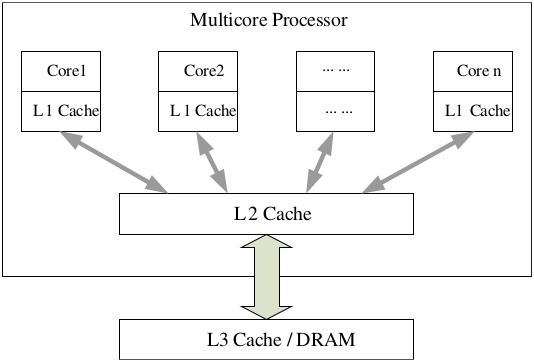
\includegraphics[width=.8\linewidth]{figures/multicore_mem}
            \end{center}
        \end{column}
    \end{columns} 
\end{frame}

%%%%%%%%%%%%%%%%%%%%%%%%%%%%%%%%%%%%%%%%%%%%%%%%%%%%%%%%%%%%%%
\section{Ley de Amdahl y eficiencia energética}
%%%%%%%%%%%%%%%%%%%%%%%%%%%%%%%%%%%%%%%%%%%%%%%%%%%%%%%%%%%%%%

\subsection*{Ley de Amdahl y eficiencia energética}

\begin{frame}{Ley de Amdahl y eficiencia energética}
    \begin{block}{Problema energético}
        \begin{itemize}
            \item El consumo energético se ha convertido en un factor clave en el diseño de las microarquitecturas.
            \begin{itemize}
                \item Establecer el impacto en el consumo eléctrico a consecuencia del aumento del número de cores.
            \end{itemize}
            \item La ley de Amdahl no contempla la energía requerida por los procesadores.
            \begin{itemize}
                \item Necesario extender la Ley de Amdahl para tener en cuenta dicho factor.
            \end{itemize}
        \end{itemize}
    \end{block}
\end{frame}

\subsection*{Estructura de los multicores en estudio}
\begin{frame}{Estructura de los multicores en estudio}
    \begin{block}{Diseños de multicores}
        Se parte de los siguientes diseños de multicores:
        \\
        \center
\includegraphics[width=.8\linewidth]{figures/amd_power_structures}
        
        \begin{itemize}
            \item a. Multicore actual. 
            \item b. Multicore basado en cores sencillos eficientes.
            \item c. Multicore asimétrico.
        \end{itemize}
    \end{block}    
    
\end{frame}

\begin{frame}{Consumo eléctrico y rendimiento en multicore actual}
    \begin{block}{Consumo eléctrico en multicore actual}
        $$ W = \frac{1 + (n - 1)k(1-f)}{(1 - f)\frac{f}{n}} $$
        \begin{itemize}
             \item $ W $ representa el consumo de energía.
             \item $ k $, perteneciente al intervalo $ [0,1] $, fracción de energía que el procesador consume en \textit{idle}.
             \item La energía consumida en secuencial por el core es 1.
                \begin{itemize}
                    \item Los $ n -1 $ cores restantes consumirán $ (n -1)k $. La fase secuencial consume $ 1 +  (n -1)k $.
                \end{itemize}
        \end{itemize}
          
    
    \end{block}
    
    
\end{frame}


\begin{frame}{Consumo eléctrico y rendimiento en multicore actual}
    \begin{block}{Rendimiento por consumo eléctrico en multicore actual}
    Partiendo de la versión simplificada de Amdahl para multicores ($ A = \frac{1}{1 - F_{mejora} + \frac{F_{mejora}}{n}} $) se obtiene el cociente:
    
        $$ \frac{Perf}{W} = \frac{1}{1 + (n - 1)k(1-f)} $$
    \\
    Gráficamente:    
    \\
    \center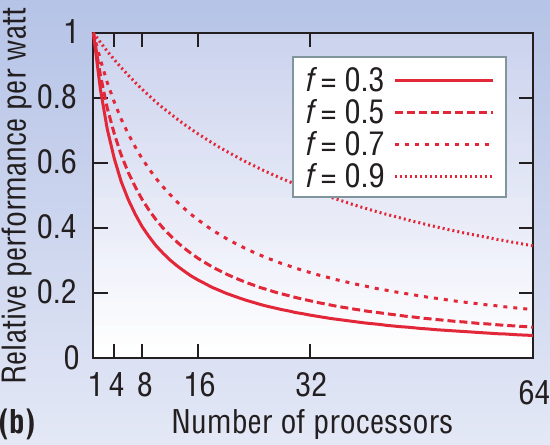
\includegraphics[width=.3\linewidth]{figures/am_powperf_a}
    
    \end{block}    
    
\end{frame}



\begin{frame}{Consumo eléctrico y rendimiento en multicore con cores sencillos eficientes}
    \begin{block}{Consumo eléctrico en multicore con cores sencillos eficientes}
        $$ W = \frac{w_{c}+ (n - 1)w_{c}k_{c}(1-f)}{(1 - f)\frac{f}{n}} $$
        \begin{itemize}
             \item $ W $ representa el consumo de energía.
             \item $ w_{c} $, en el intervalo $ [0,1] $, representa el consumo relativo de un core sencillo activo frente a un procesador completo.
             \item Análogamente, $ k_{c} $, en el intervalo $ [0,1] $, representa el consumo normalizado de un core sencillo en \textit{idle} frente a un procesador completo.
             \item La energía consumida en secuencial por el core sencillo es $ w_{c} $.
                \begin{itemize}
                    \item Los $ n -1 $ cores restantes consumirán $ (n -1)w_{c}k_{c} $. La fase secuencial consume $ n w_{c} $.
                \end{itemize}
        \end{itemize}
          
    
    \end{block}
    
    
\end{frame}


\begin{frame}{Consumo eléctrico y rendimiento en multicore con cores sencillos}
    \begin{block}{Rendimiento por consumo eléctrico en multicore con cores sencillos}
    Partiendo de la versión simplificada de Amdahl para multicores ($ A = \frac{s_{c}}{1 - F_{mejora} + \frac{F_{mejora}}{n}} $) se obtiene el cociente:
    
        $$ \frac{Perf}{W} = \frac{s_{c}}{w_{c} + (n - 1)w_{c}k_{c}(1-f)} $$
    donde $ s_{c} $ (en $ [0,1] $) representa el rendimiento de un core sencillo normalizado al rendimiento de un procesador completo. Gráficamente:    
    \center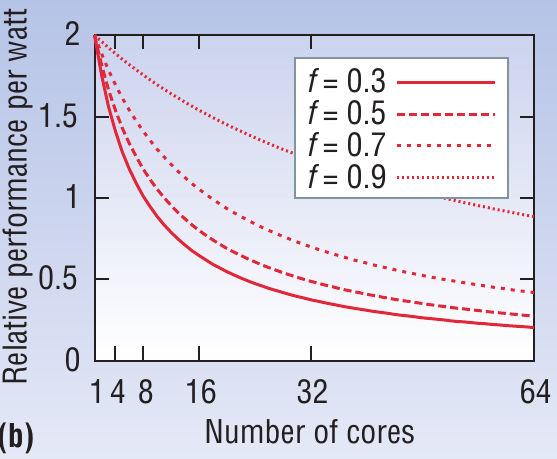
\includegraphics[width=.25\linewidth]{figures/am_powperf_b}
    
    \end{block}    
    
\end{frame}


\begin{frame}{Consumo eléctrico y rendimiento en multicore asimétrico}
    \begin{block}{Consumo eléctrico en multicore asimétrico}
        $$ W = \frac{(1 -f)(1+(n-1)w_{c}k_{c}) + \frac{f}{s_{c}} (\frac{k}{n-1} + w_{c})}{(1 - f)\frac{f}{(n-1)s_{c}}} $$
        \begin{itemize}
             \item $ k $, en $ [0,1] $, fracción de energía que el core completo consume en la fase paralela.

        \end{itemize}
          
    
    \end{block}
    
    
\end{frame}


\begin{frame}{Consumo eléctrico y rendimiento en multicore asimétrico}
    \begin{block}{Rendimiento por consumo eléctrico en multicore asimétrico}
    Partiendo de la versión simplificada de Amdahl para multicores ($ A = \frac{1}{1 - F_{mejora} + \frac{F_{mejora}}{n}} $) se obtiene el cociente:
    
        $$ \frac{Perf}{W} = \frac{1}{(1-f)(1+(n-1)w_{c}k_{c}) + \frac{f}{s_{c}} (\frac{k}{n-1} + w_{c})} $$
    \\
    Gráficamente:    
    \\
    \center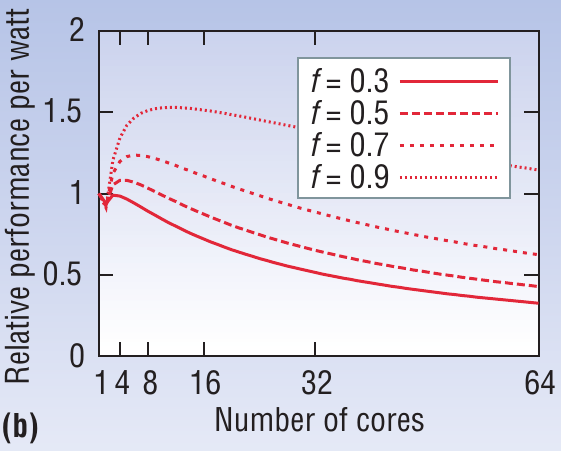
\includegraphics[width=.3\linewidth]{figures/am_powperf_c}
    
    \end{block}    
    
\end{frame}


\begin{frame}{Comparativa rendimiento por consumo}
    \begin{block}{Comparativa rendimiento por consumo}
\center
    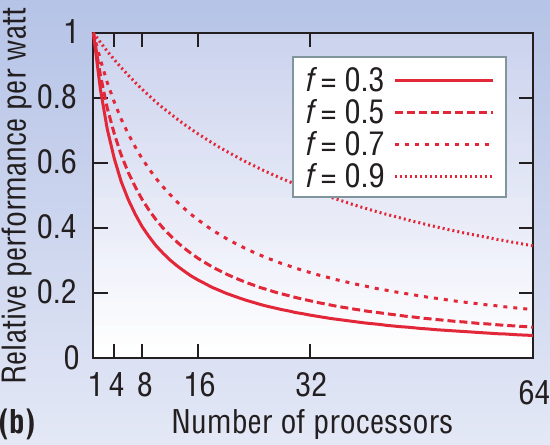
\includegraphics[width=.3\linewidth]{figures/am_powperf_a}
    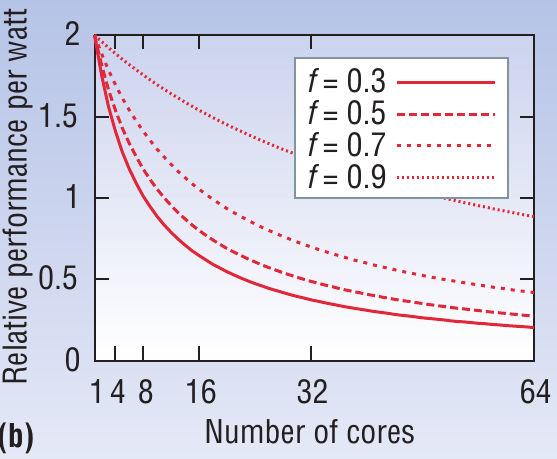
\includegraphics[width=.3\linewidth]{figures/am_powperf_b}
    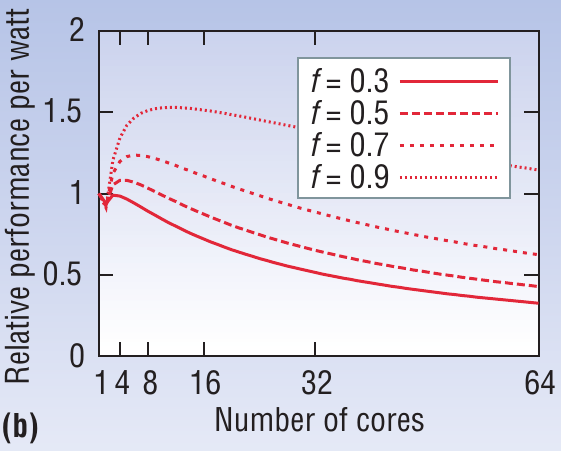
\includegraphics[width=.3\linewidth]{figures/am_powperf_c}
    \end{block}    
    
\end{frame}




%%%%%%%%%%%%%%%%%%%%%%%%%%%%%%%%%%%%%%%%%%%%%%%%%%%%%%%%%%%%%%
\section{Bibliografía}
%%%%%%%%%%%%%%%%%%%%%%%%%%%%%%%%%%%%%%%%%%%%%%%%%%%%%%%%%%%%%%

\begin{frame}[allowframebreaks]{Bibliografía}
    \nocite{*}
    \bibliographystyle{pfc-fic}
    \bibliography{biblio}
\end{frame}

\end{document}
